\section{From Candidates to Program}

    The way we approach this is to not have any assumptions as to why the compiler chooses to do a particular reordering in the program. 
    We instead only check if the reoredered program can have its observable behaviors as a subset of the original. 
    This ensures that the algorithm for the compiler optimization need not change, but that our set of conditions will just be additional checks that can be done before actually doing the reordering. 
    Such an approach makes reordering parametric to the memory model. 
    
    The downside is that this approach will be conservative as we use no information as to why a particular set of events are reordered. We do not compare and contrast in details the perks of both approaches. This is beyond the scope of this thesis.

    \subsection{Addressing Programs with Conditionals}
        We first consider the elimination of write in programs with conditional branches. The following corollary states when doing such an elimination is safe: 

        \begin{corollary}
            Consider a program $P$ and its candidates $C_1, C_2, ... , C_n$ in which events $e$ and $d$ present such that 
            \begin{align*}
                \event{e}{W} \ \wedge \ \event{d}{W} \ \wedge \ \et{e}{uo} \ \wedge \ \reln{e}{ao}{d} \ \wedge \ \Re(e)\!=\!\Re(d)
            \end{align*} . 
            Consider the set of corresponding candidates $C'_1, C'_2, ... , C'_n$ after eliminating $e$ and its corresponding program $P'$. If
            \begin{align*}
                \forall C_{i \in [1,n]}, \forall k \in C_i \ \text{s.t.} \ \reln{e}{ao}{k} \wedge \reln{k}{ao}{d}, \    
                Reord(e,k)  
            \end{align*}
            and
            \begin{align*}
                \nexists C \in P \ \text{s.t.} \ \event{e}{C} \wedge d \notin C
            \end{align*}
            Then the set of observable behaviors of $P'$ is a subset of that of $P$.
        \end{corollary}

        \begin{proof}
            We first prove that the second condition must hold. We show this by proving that if it does not hold, a new observable behavior     can be introduced. 

            Suppose the second condition does not hold, then we have 
            \begin{align*}
                \exists C \in P \ \text{s.t.} \  \event{e}{C} \wedge d \notin C
            \end{align*}

            By Prop \ref{CondB1} and Prop \ref{CondB1}, we can infer that the above holds if $e$ or $d$ are part of a conditional branch. 
            \begin{itemize}
                \item Case 1: $e$ and $d$ both are part of conditionals 

                    If $e$ and $d$ are part of different branches of the same conditional, then we have $\neg \reln{e}{ao}{d}$. Hence this  case need not be considered.     

                    There are remaining four types of this case that we need to consider: 

                    \begin{enumerate}
                        \item Type 1: 

                            \begin{figure}[H]
                                \centering 
                                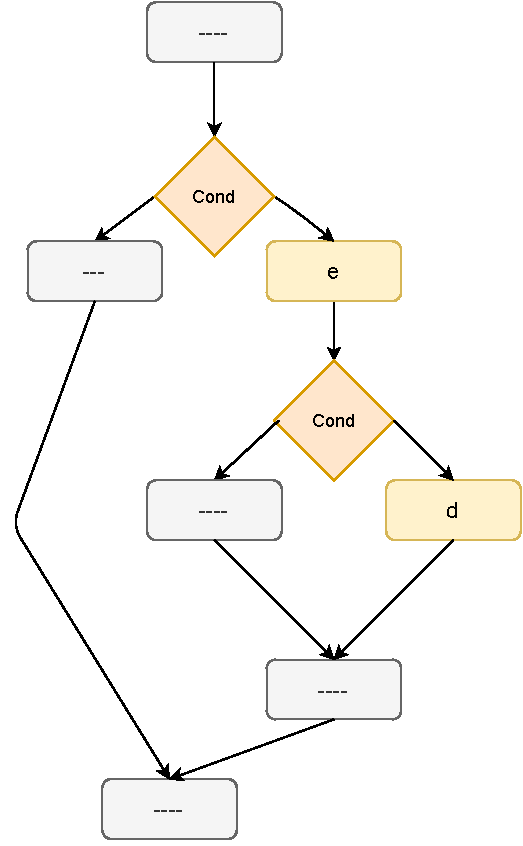
\includegraphics[scale=0.7]{Elimination/ConditionalsProofFig1.pdf}
                                \caption{Type 1:}    
                            \end{figure}
                        
                            From the figure, we can infer by Prop \ref{CondB1} that  
                            \begin{align*}
                                \exists C \in P \ \text{s.t.} \ e \in C \ \wedge \ d \notin C
                            \end{align*}
                            After elimination $e$, we can have a new observable behavior in a candidate not having $d$ from the above property of this case.  

                        \item Type 2: 

                            \begin{figure}[H]
                                \centering 
                                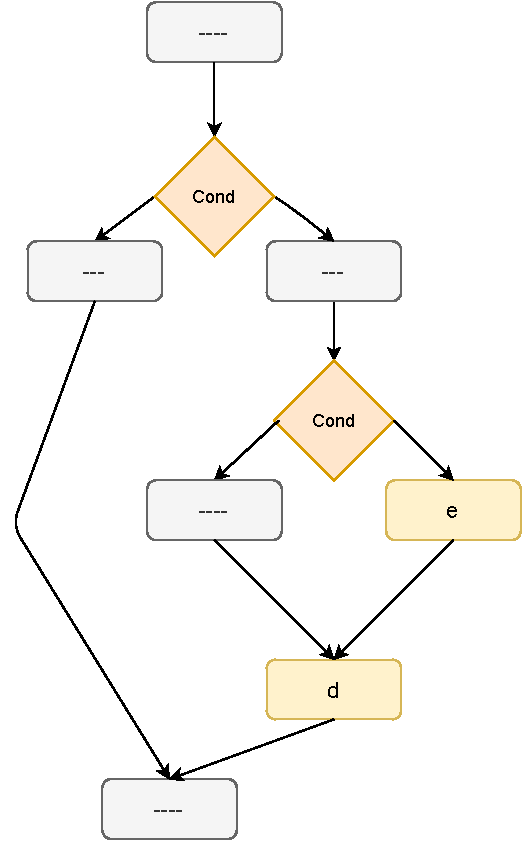
\includegraphics[scale=0.7]{Elimination/ConditionalsProofFig2.pdf}
                                \caption{Type 2:}    
                            \end{figure}
                        
                            From the figure, we can infer by Prop \ref{CondB1} that
                            \begin{align*}
                                \exists C \in P \ \text{s.t.} \ e \notin C \ \wedge \ d \in C
                            \end{align*}
                            After elimination $e$, we cannot have any new observable behavior in a candidate not having $d$ as by Prop \ref {CondB1}, we have for the original program that  
                            \begin{align*}
                                \exists C \in P \ \text{s.t.} \ e \notin C \ \wedge \ d \notin C
                            \end{align*}

                        \item Type 3: 
                        
                            \begin{figure}[H]
                                \centering 
                                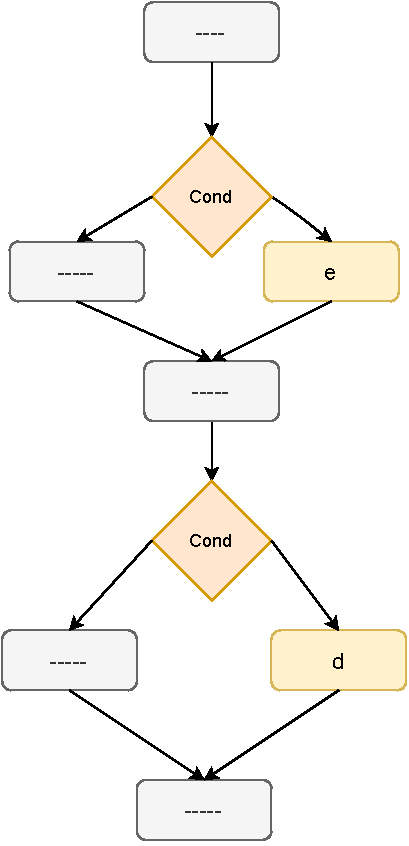
\includegraphics[scale=0.7]{Elimination/ConditionalsProofFig3.pdf}
                                \caption{Type 3:}    
                            \end{figure}

                            If $e$ and $d$ are part of different conditional branches, then by Prop \ref{CondB2} and \ref{CondB1}, we have 
                            \begin{align*}
                                \exists C \in P \ \text{s.t.} \ d \notin C \\ 
                                \exists C \in P \ \text{s.t.} \ e \notin C 
                            \end{align*}
                            After elimination $e$, we can have a new observable behavior in a candidate not having $d$ as above condition states. 
                        
                        \item Type 4: 

                            \begin{figure}[H]
                                \centering 
                                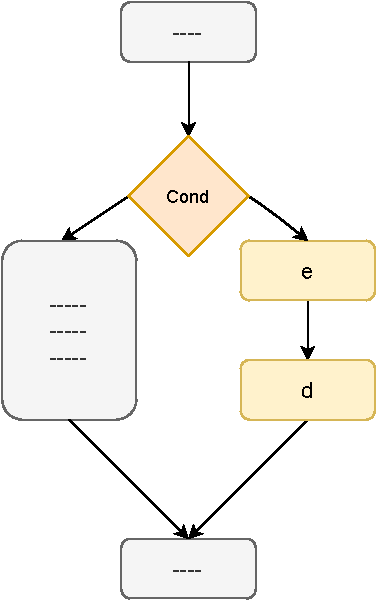
\includegraphics[scale=0.7]{Elimination/ConditionalsProofFig4.pdf}
                                \caption{Type 4:}    
                            \end{figure}

                            From the figure, we can infer by Prop \ref{CondB1} that
                            \begin{align*}
                                \exists C \in P \ \text{s.t.} \ e \notin C \ \wedge \ d \notin C
                            \end{align*}
                            After elimination $e$, we cannot have any new observable behavior in a candidate not having $d$ as we have by Prop \ref{CondB1} that  
                            \begin{align*}
                                e \in C \ \Rightarrow \ d \in C
                            \end{align*}

                            \critic{purple}{Not sure how to come to the above conclusion apart from the fact that its obvious.}

                    \end{enumerate}

                    \critic{red}{Need to refer to part of elimination proof as Coherent Reads would not be triggered anymore for a case and thus we can have a new observable behavior. How to explain this, ask Clark.}

                \item Case 2: $e$ is part of conditional but $d$ is not

                    \begin{figure}[H]
                        \centering 
                        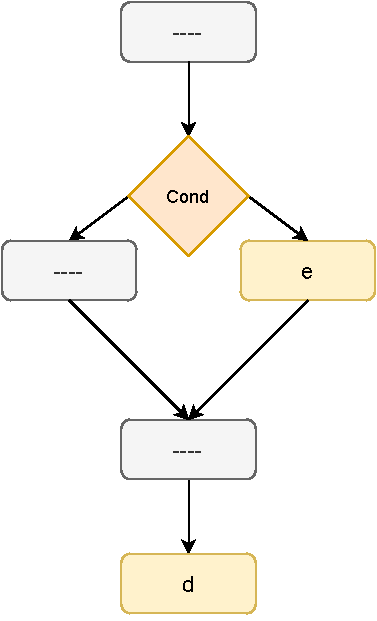
\includegraphics[scale=0.7]{Elimination/ConditionalsProofFig6.pdf}
                        \caption{ }    
                    \end{figure}
                
                
                    By Prop \ref{CondB2} and \ref{CondB1}, we have 
                    \begin{align*}
                        \exists C \in P \ \text{s.t.} \ e \notin C 
                    \end{align*}
                    After elimination $e$, we cannot have a new observable behavior in a candidate due to not having $d$ as above condition states.

                \item Case 3: $d$ is part of a conditional but $e$ is not

                    \begin{figure}[H]
                        \centering 
                        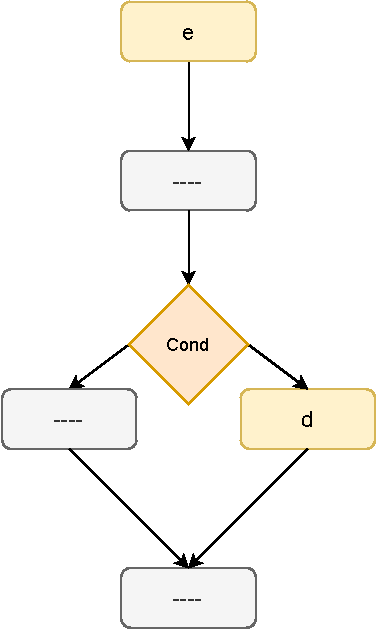
\includegraphics[scale=0.7]{Elimination/ConditionalsProofFig5.pdf}
                        \caption{4:}    
                    \end{figure}

                    By Prop \ref{CondB2} and \ref{CondB1}, we have 
                    \begin{align*}
                        \exists C \in P \ \text{s.t.} \ d \notin C
                    \end{align*}
                    After elimination $e$, we can have a new observable behavior in a candidate not having $d$ as above condition states. 

                    \critic{red}{Need to refer to part of elimination proof as Coherent Reads would not be triggered anymore for a case and thus we can have a new observable behavior. How to explain this, ask Clark.}

                    \critic{purple}{Add the above property to conditionals with two branches also.}

            \end{itemize}

            Now that we have that the second condition must hold, we prove the first condition too must hold. Let $C_i$ and $C_i'$ be the candidates before and after eliminating $e$. From the first condition we have then for $C_i$
            \begin{align*}
                \forall \ k \ \textit{s.t.} \ 
                \reln{e}{ao}{k} \ \wedge \ \reln{k}{ao}{d} \ . \ 
                Reord(e,k).
            \end{align*}
            The above is Corollary 1 (tag properly) for elimination, thus giving us that the observable behaviors of $C_i'$ is a subset of $C_i$. Hence this condition must hold for all candidates from which we eliminate $e$. 

            By property of unions of sets, we can conclude that the set of Observable Behaviors of $P'$ is a subset of that of $P$.

            Hence proved.

            \critic{purple}{We have not given properly the link between Observable Behaviors, Candidate Executions, Candidates and Programs. Perhaps we need to define a function Obs that gives us the set of Observable Behaviors, where the Domain can be a Program, Candidate, or Candidate Execution.}
    \end{proof}

        As far as read elimination goes, since we only need the information of read event that is to be eliminated, we do not need to take cases as above for write elimination. Except there can exist one case, in which the read itself is the conditional check. But what is the resultant code after elimination relies on the intention of the compiler, which can be the following:
        \begin{itemize}
            \item It could be plain dead code elimination, wherein both brnaches of code are eliminated entirely. 
            \item It could also be that the conditonal check always returns the same value, which makes the branch taken to be the same. 
            \item It could also be that the choice of branch does not affect the outcome of the program itself. 
        \end{itemize}
    
        Since we aren't certain of the reason, it is difficult to identify the target code that is inteneded after such an elminiation. Hence we do not address this case. It is also not within the scope of our analysis to conhsder the actual mapping between program and candidates. We would need this to prove that the program does not take a particular conditonal branch in any execution. This is not easy to do without the mapping in our hands. 


    \subsection{Addressing Programs with Loops}
    
        Similar to reordering, for the sake of elimination, we consider programs with just one loop. 
        
        We first consider the simpler case of read elimination within a loop. 
        Eliminating such a read at a program level would imply in every candidate $C^i$ where $i$ denotes the number of iterations, the read $R$ within the loop can be eliminated.
        
        By Thereom 1 of read elimination, we only need the read $R$ to have the type $uo$ to perform such an elimination.
        Thus we can eliminate for each iteration of the loop our intended read. 
        By transitive property of subsets, the resultant candidate will have observable behaviors as a subset of the original. 
        Doing this for all valid canddiates extends to program level.

        Next we consider the case of eliminating writes within a loop. 
        Eliminating such a read at a program level would imply in every candidate $C^i$ where $i$ denotes the number of iterations, the read $W$ within the loop can be eliminated.

        For this, we need to have some write $d$ that can exist in all candidates where $e$ can exist. ($\nexists C \in P \ \text{s.t} \ e \in C \wedge d \notin C$). This condition corresponds to Corollary 2 of elimination, which handles the case of conditonals too. 
        Next, we need to show that in each iteration the write $e$ can be eliminated. We once again have Corollary 2 to show when we can do this. 
        By transitive property of subsets, we can show that the resultant candidate has observable behaviors as a subset of original. 
        Doing this for all valid canddiates extends to program level.
         

        \paragraph{Loop Invariant Code motion}  

            In the previous chapter, we showed that loop invariant code motion cannot be validated by just reordering at the Candidate level. 
            This was because reordering was insufficient to generate the resultant candidate from the original. 
            This however can be done by coupling Reordering with Elimination. 
            
            We first consider the case of reordering a Read outside a loop.
            \begin{itemize}          
                  \item  We have two subcases of this; one with reordering it before the loop and the one after.
                    For both subcases note that we need to have just one Read in the resultant candidate irrespective of the number of iterataions of the loop. 
                \item Thus, we need to show that for any Candidate  $C^i$ of the original program, we can eliminate $i-1$ reads and reorder the remaining one to be outside the loop. 
                \item The main question then comes is which read is to be chosen for this? Does it matter which iteration's read is chosen to be kept? It turns out that it matters when we do not choose the last read in every iteration.  
                \item We can show that retaining the first iteration's read is not safe to do by constructing a simple counter example for it. 
                \item We can show similarly a counterexample for retaining any read of some random iteration which is not the last. 
                \item But how can we assert which is the last iteration? Since we place no bounds on the number of iterations a loop can have, this is not possible. 
                \item However, we have the set of events that can occur between two reads of consecutive iterations. From the property of Reord under loops between events of different iterations, it suffices to show that if  $Reord(k, R)$ holds for every such event $k \in K$, no matter how many iterations, we can always reorder the last iteration's read $R$ to be above the loop. 
                \item This helps us skip the complexity of dealing with deciding which iteration's read should be considered last, and skips the complexity of iterations entirely. 
                \item Because we have $Reord(k, R)$, no matter what iteration it is, we can always reorder the last read. 
            \end{itemize}

            \begin{itemize}
                \item An alternative way of proving this is to show that we can reorder each iterative read, to be consecutive to each other $cons(R^i, R^{i+i})$. In doing so we can ensure that we can safely eliminate the reads. 
                \item Because the reads are of type $uo$, having them consecutive to each other will then play a role of it being representative of just one read. 
                \item Hence, we can eliminate all but one read. 
                \item This will help avoid dealing with which iteration's read to be chosen for elimination. 
                \item Once again, we need to show that for any event $k \in K$ we have $Reord(k, R)$. This will ensure that irrespective of the iteration, we can always have reads between two consecutive iterations to be consecutive in a candidate due to successive reordering.
                \item Corollary of code motion in candidates help us show this in terms of observable behaviors.
            \end{itemize}

            Now we consider the case of reordering a write outside a loop:
             
            \begin{itemize}
                \item We again have two subcases for this; one with reordering it before the loop and the one after. 
                \item In each case, the common requirement is that irrespective of the iterations of the loop, only one write should exist in each candidate.
                \item Note that when we have more than one iteration of the loop, we have two writes, out of which one must be eliminated. 
                \item For instance, given candidate $C^2$, should we eliminate $w^1$ or $w^2$? 
                \item We can from Corollary of write elimination assert when we can remove $w^1$. However, if we want to elimiante $w^2$, we would need information of the existance of some other write either within or outside the same loop, program ordered after $w^2$. 
                \item Getting such information would require another flow analysis. But more importantly, suhc informaion is not alwyas required in the sequential programs to assert loop invariant code motion. Though the choice remains. 
                \item Without having information of the existance of such a write, we can consider eliminating $w^1$, which would firstly require $Reord(w^1, k)$ where $\reln{w^1}{ao}{k} \wedge \reln{k}{ao}{w^2}$. 
                \item We can extend the above requirement to incorporate elimination under conditionals using Corollary 2 for write elimination. 
                \item Thus in general for any Candidate $C^i$, we require that all $w^{j<i}$ be eliminable. To prove this requirement Corollary 2 suffices.
                \item We must also note that if $w^j$ in general is part of a conditonal branch, then we cannot eliminate it mainly because it also represents the same event $d$ using whose reference we can safely consider eliminating $w^j$. 
                \item Doing such successive elimination leaves $w^i$ for every such $C^i$. 
                \item Now based on each subcase, we require either $Reord(k, w^i)$ or $Reord(w^i, k)$ to hold for an event $k$ existing in the loop. Npte that for the first subcase, we need all the events within the loop to be considered reorderable with $w^i$. But for the second, we only need the events that are after $w$ in the loop. 
                \item For both cases, we have the base argument that $k$ can be agent ordered with the wrtie $w^i$. So all such agent ordered events $k$ have to be considered if they need to be reorrdered with $w^i$. 
                \item Proving this is again by Corollary 2 of write elimination. Though note that we will also need code motion corollaries from reordering for this.  
            \end{itemize}


        \paragraph{Reordering two events accross loops} 
            
            Note that we still cannot assert when we can reorder events inside a loop. This would require a proof of redundancy introduction at the candidate level. While this can be done, this is outside the scope of this thesis and is kept as part of future work. But for now, we will show a counter example as to why such reordering is not always safe to do. 

            \critic{blue}{One for reordering Reads}

            \critic{blue}{One for reordering Write-Read}

            \critic{blue}{One for reordering Read-Write}

            \critic{blue}{One for reordering Write-Write}

            For each of the above examples, we note that it is not safe to perform such reordering in general. 